Dieses Projekt entsteht im Zusammenhang mit einer Schularbeit. Der Fokus liegt primär auf dem Lerninhalt und der Umsetzung. Die Eignung und Verwendbarkeit des Resultats ist sekundär.

\section{Projektinhalt}
Ziel ist es, für ein kleines fiktives Unternehmen, welches Speisen wie Fast Food und ähnliche Snacks verkauft, eine Kassenverwaltungssoftware zu implementieren, die den Verkauf analysiert und das Lager verwaltet.
Bisher wurden die Arbeiten ohne Verwaltungssystem durchgeführt und die Kassierung erfolge manuell.
Dadurch herrscht ein höherer Aufwand für Kassenbuch, Steuerberater und die Verwaltung der liquiden Mittel.
Bei Einnahmezählungen kann nicht festgestellt werden, welche Produkte sich am besten Verkauft haben und ob es sich Einnahmen mit Ausgaben decken.

Besonderen Wert soll darauf gelegt werden, dass die Software ohne großen Einarbeitungsaufwand bedient und durch die Verwendung einen modernen Technologiestacks in Zukunft einfach gewartet und verwendet werden kann.
Da es sich um ein Kassensystem handelt, sind die Anforderungen an Datensicherheit und -integrität besonders hoch.

\section{Erwartungshorizont}
Die bereits vorhandene Infrastruktur basiert auf Windows 10 Computern der x64-Architektur.
Daher muss die Anwendung mit mindestens Windows 10 oder neuer kompatibel sein.
Eine Netzwerkfähigkeit muss gewährleistet sein, um den Datenaustausch über das interne Netzwerk zu ermöglichen.
Im Verwaltungsbereich sollen Mitarbeiter Einnahmen und Produkte verwalten können.
Genannte Produkte sollen sinnvolle Eigenschaften wie Bezeichnung, Einzelpreis, Verfügbarkeit im Lager besitzen.
Die getätigten Transaktionen sollen als Statistik gespeichert und dargestellt werden, um dem Benutzer einen Überblick über die vergangenen Verkäufe zu geben.
Dabei soll die Darstellung der Daten vorerst nicht erfolgen, d.\,h., die Entwicklung eines Clients (etwa in Form einer GUI) ist nicht Teil des Projekts.
Die Verarbeitung der Anfragen und Daten erfolgt über eine API, die Endpunkte für die benötigten Funktionen bieten, welche von Clients frei verwendet werden können.
Ein Client ist jedoch nicht Teil des Erwartungshorizonts.
Das Projekt muss im Zeitraum vom 27.12.2022 bis 13.03.2023 fertiggestellt werden.
Eine finanzielle Begrenzung gibt es nicht.

\section{Zeitliche Planung}
Den Abbildungen \vref{gantt1}, \vref{gantt2} und \vref{gantt3} kann die zeitliche Planung entnommen werden. Sie stellen ein Gantt-Diagramm dar, welches einen Überblick über den Aufwand des Projektes verschaffen soll und als Orientierungshilfe gilt, wenn es um das Zeitmanagement geht.

\begin{sidewaysfigure}[ht]
	\centering
	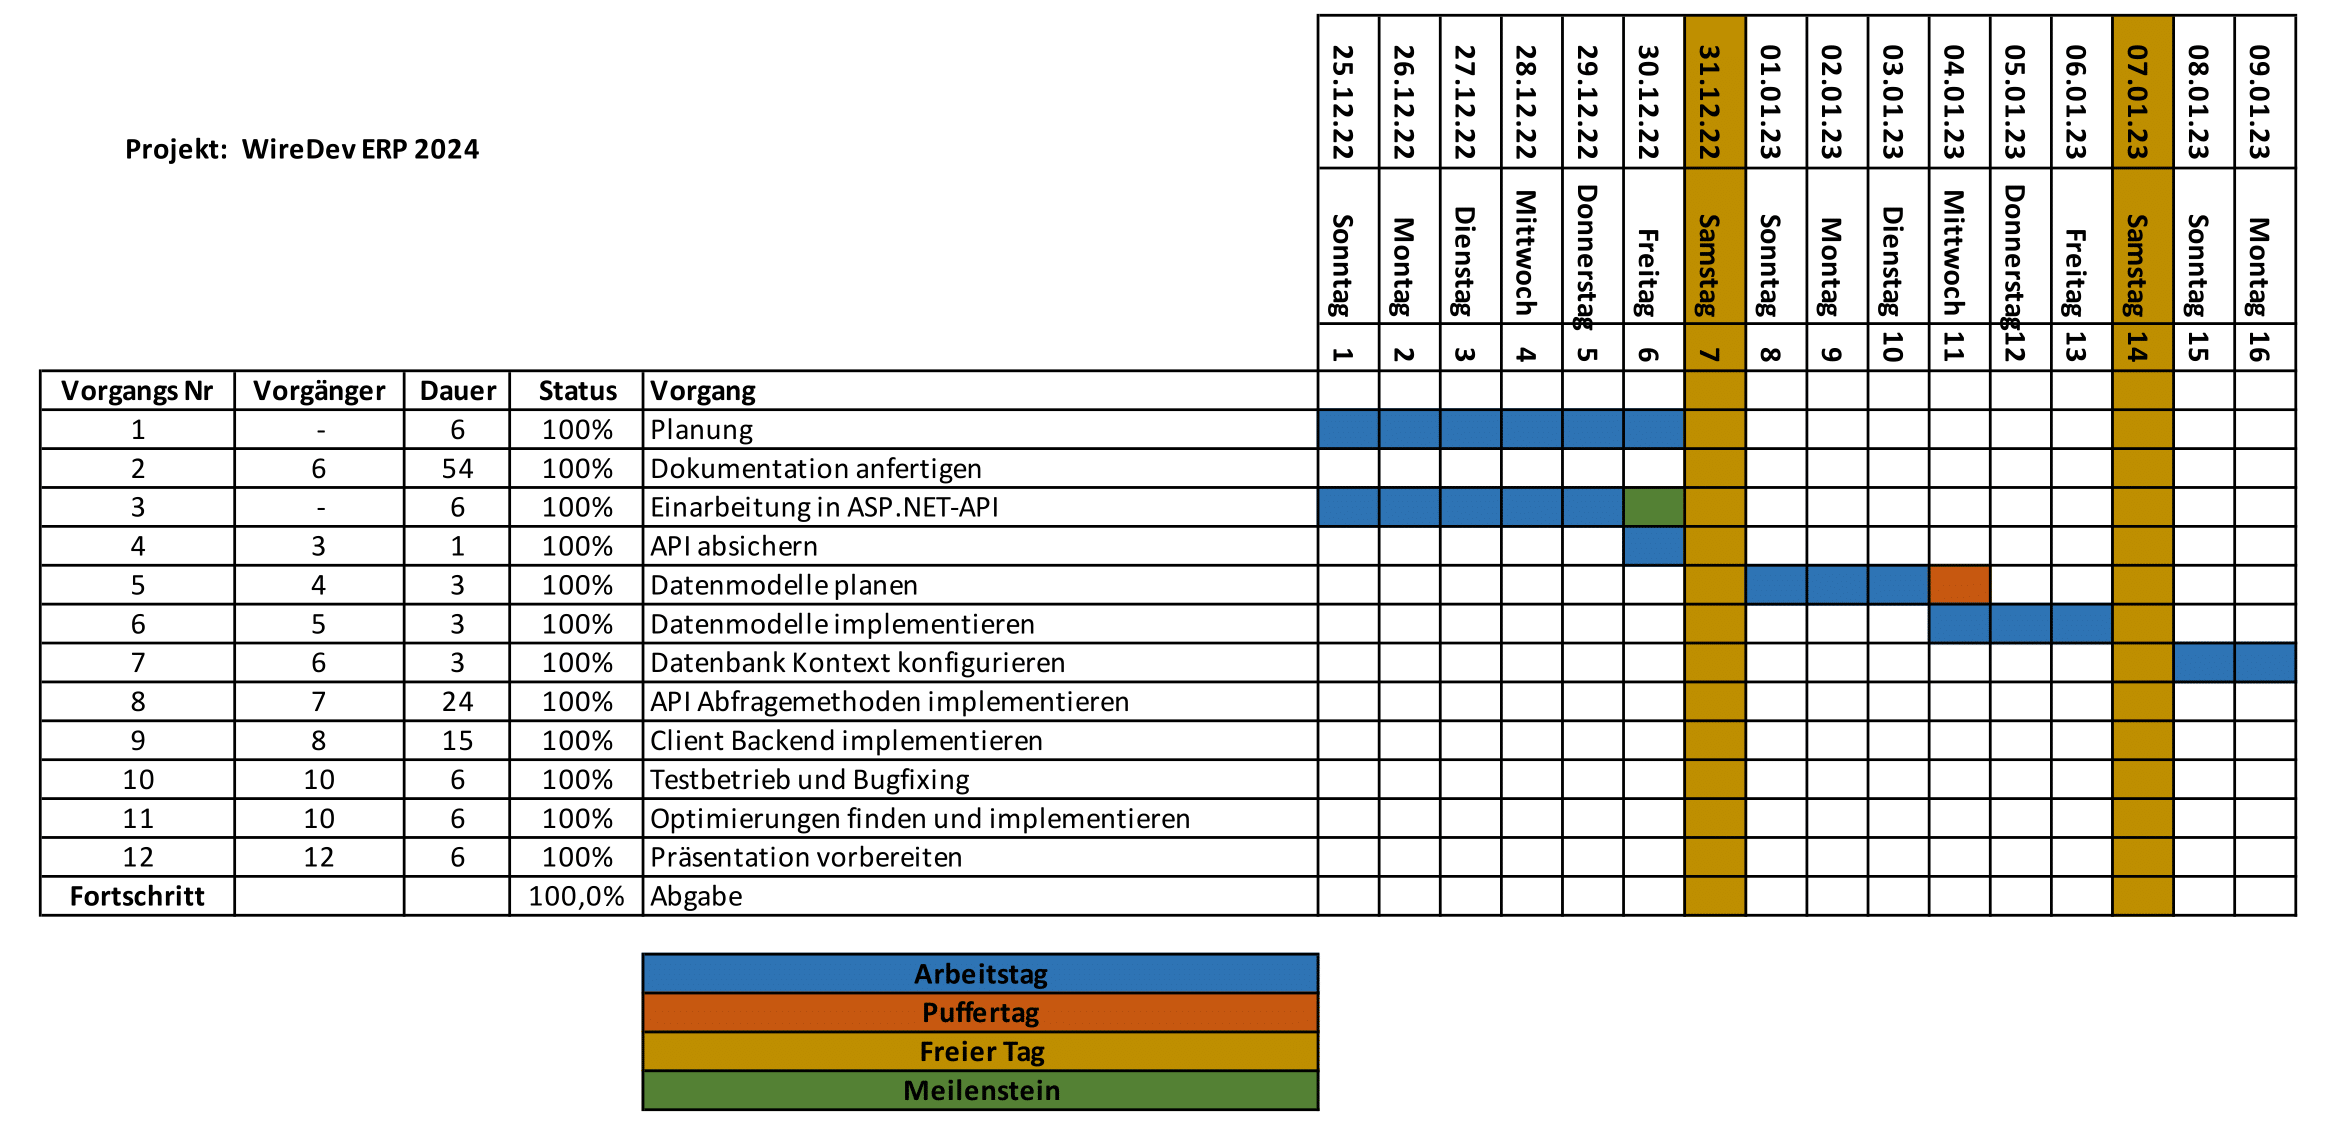
\includegraphics[width=1\linewidth]{Gantt-1.png}
	\caption{Zeitliche Planung Teil 1/3}
	\label{gantt1}
\end{sidewaysfigure}

\begin{sidewaysfigure}[ht]
\centering
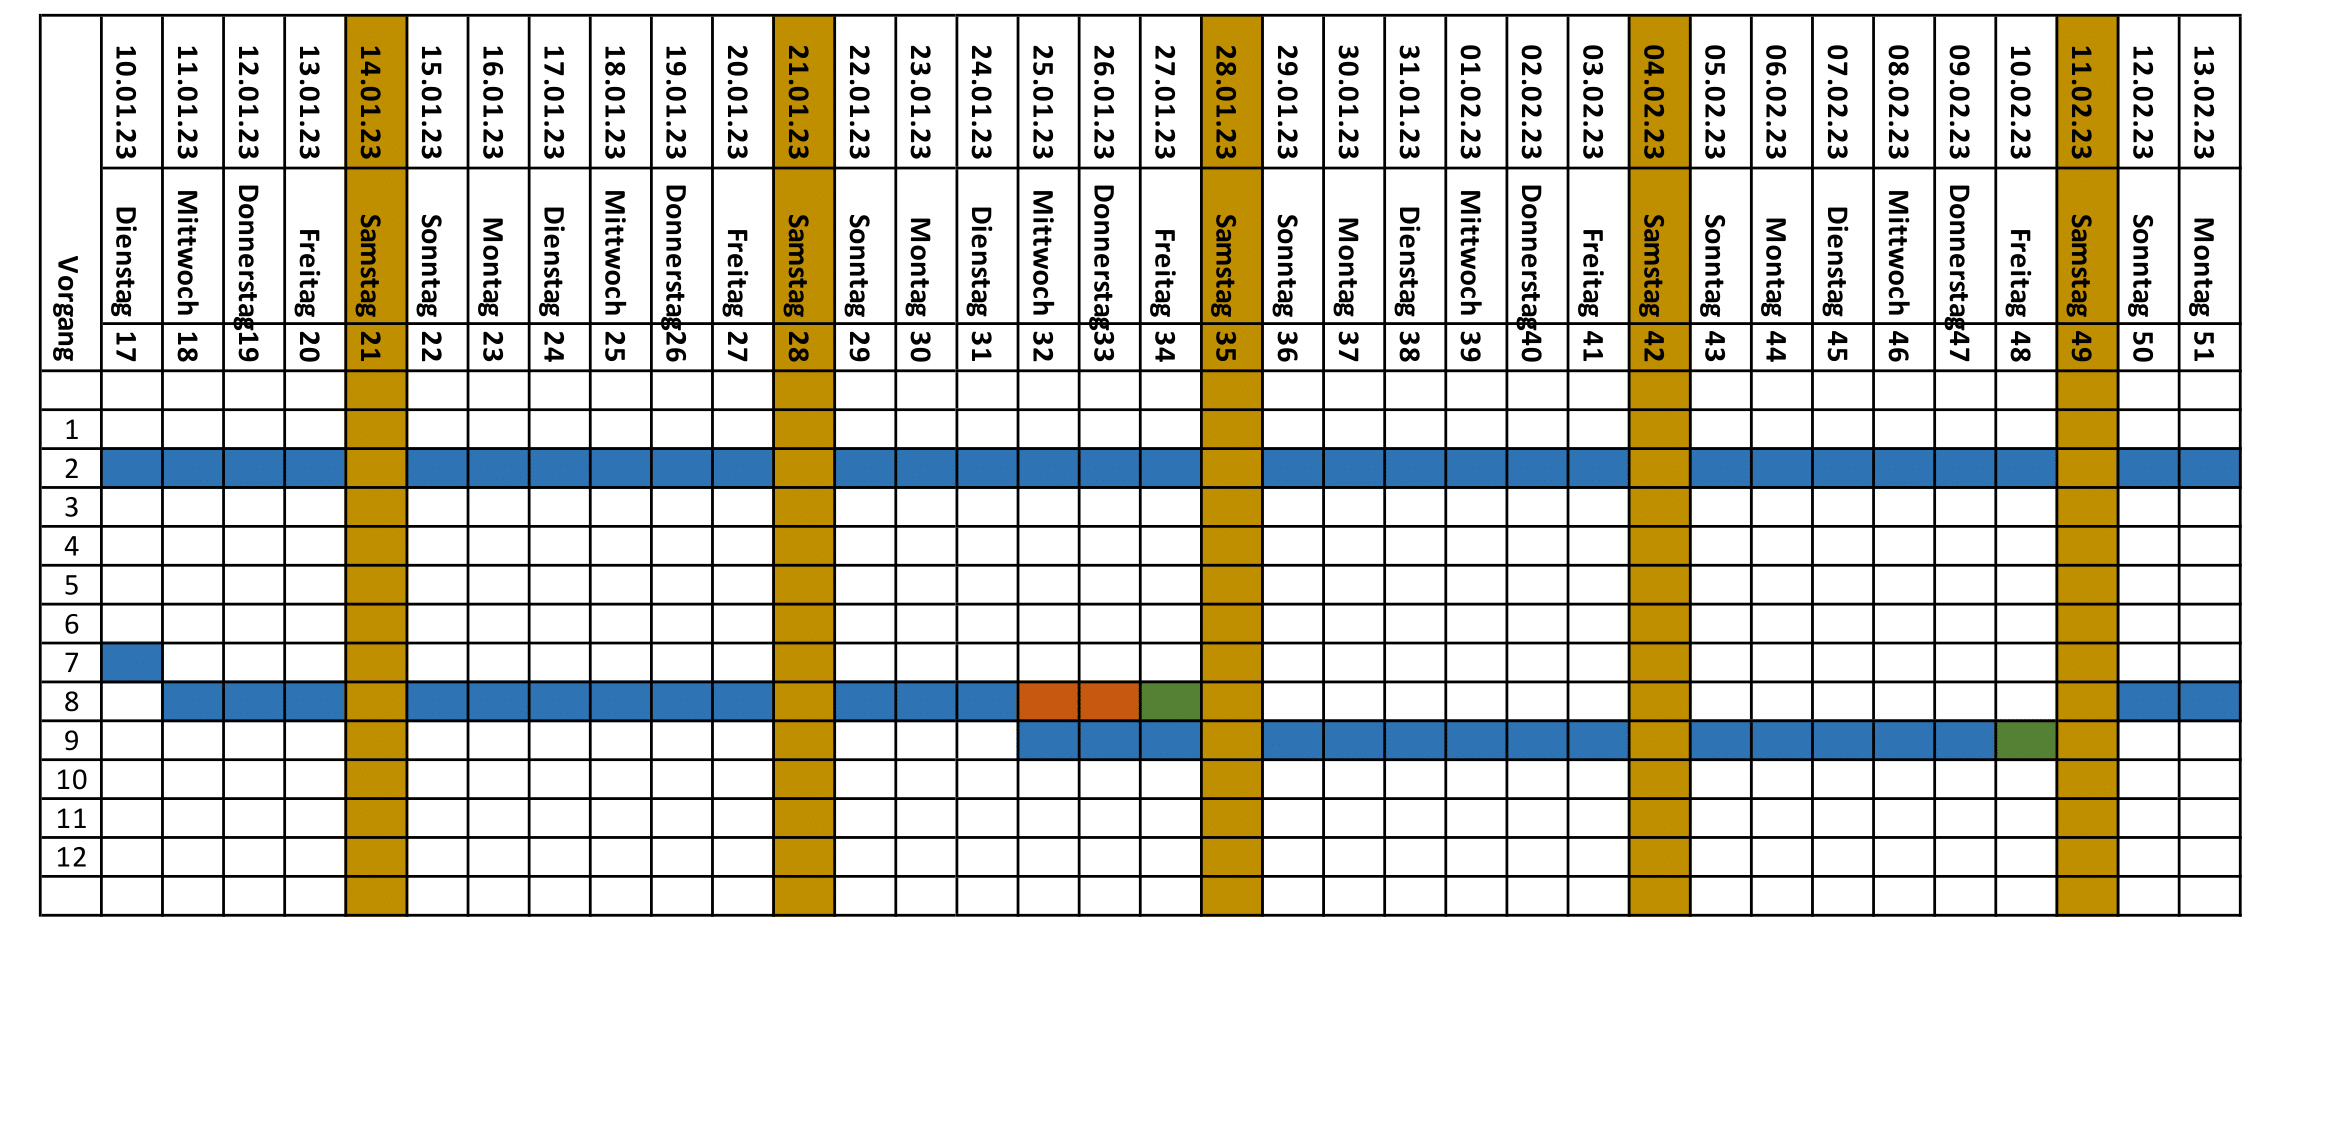
\includegraphics[width=1\linewidth]{Gantt-2.png}
\caption{Zeitliche Planung 2/3}
\label{gantt2}
\end{sidewaysfigure}

\begin{sidewaysfigure}[ht]
\centering
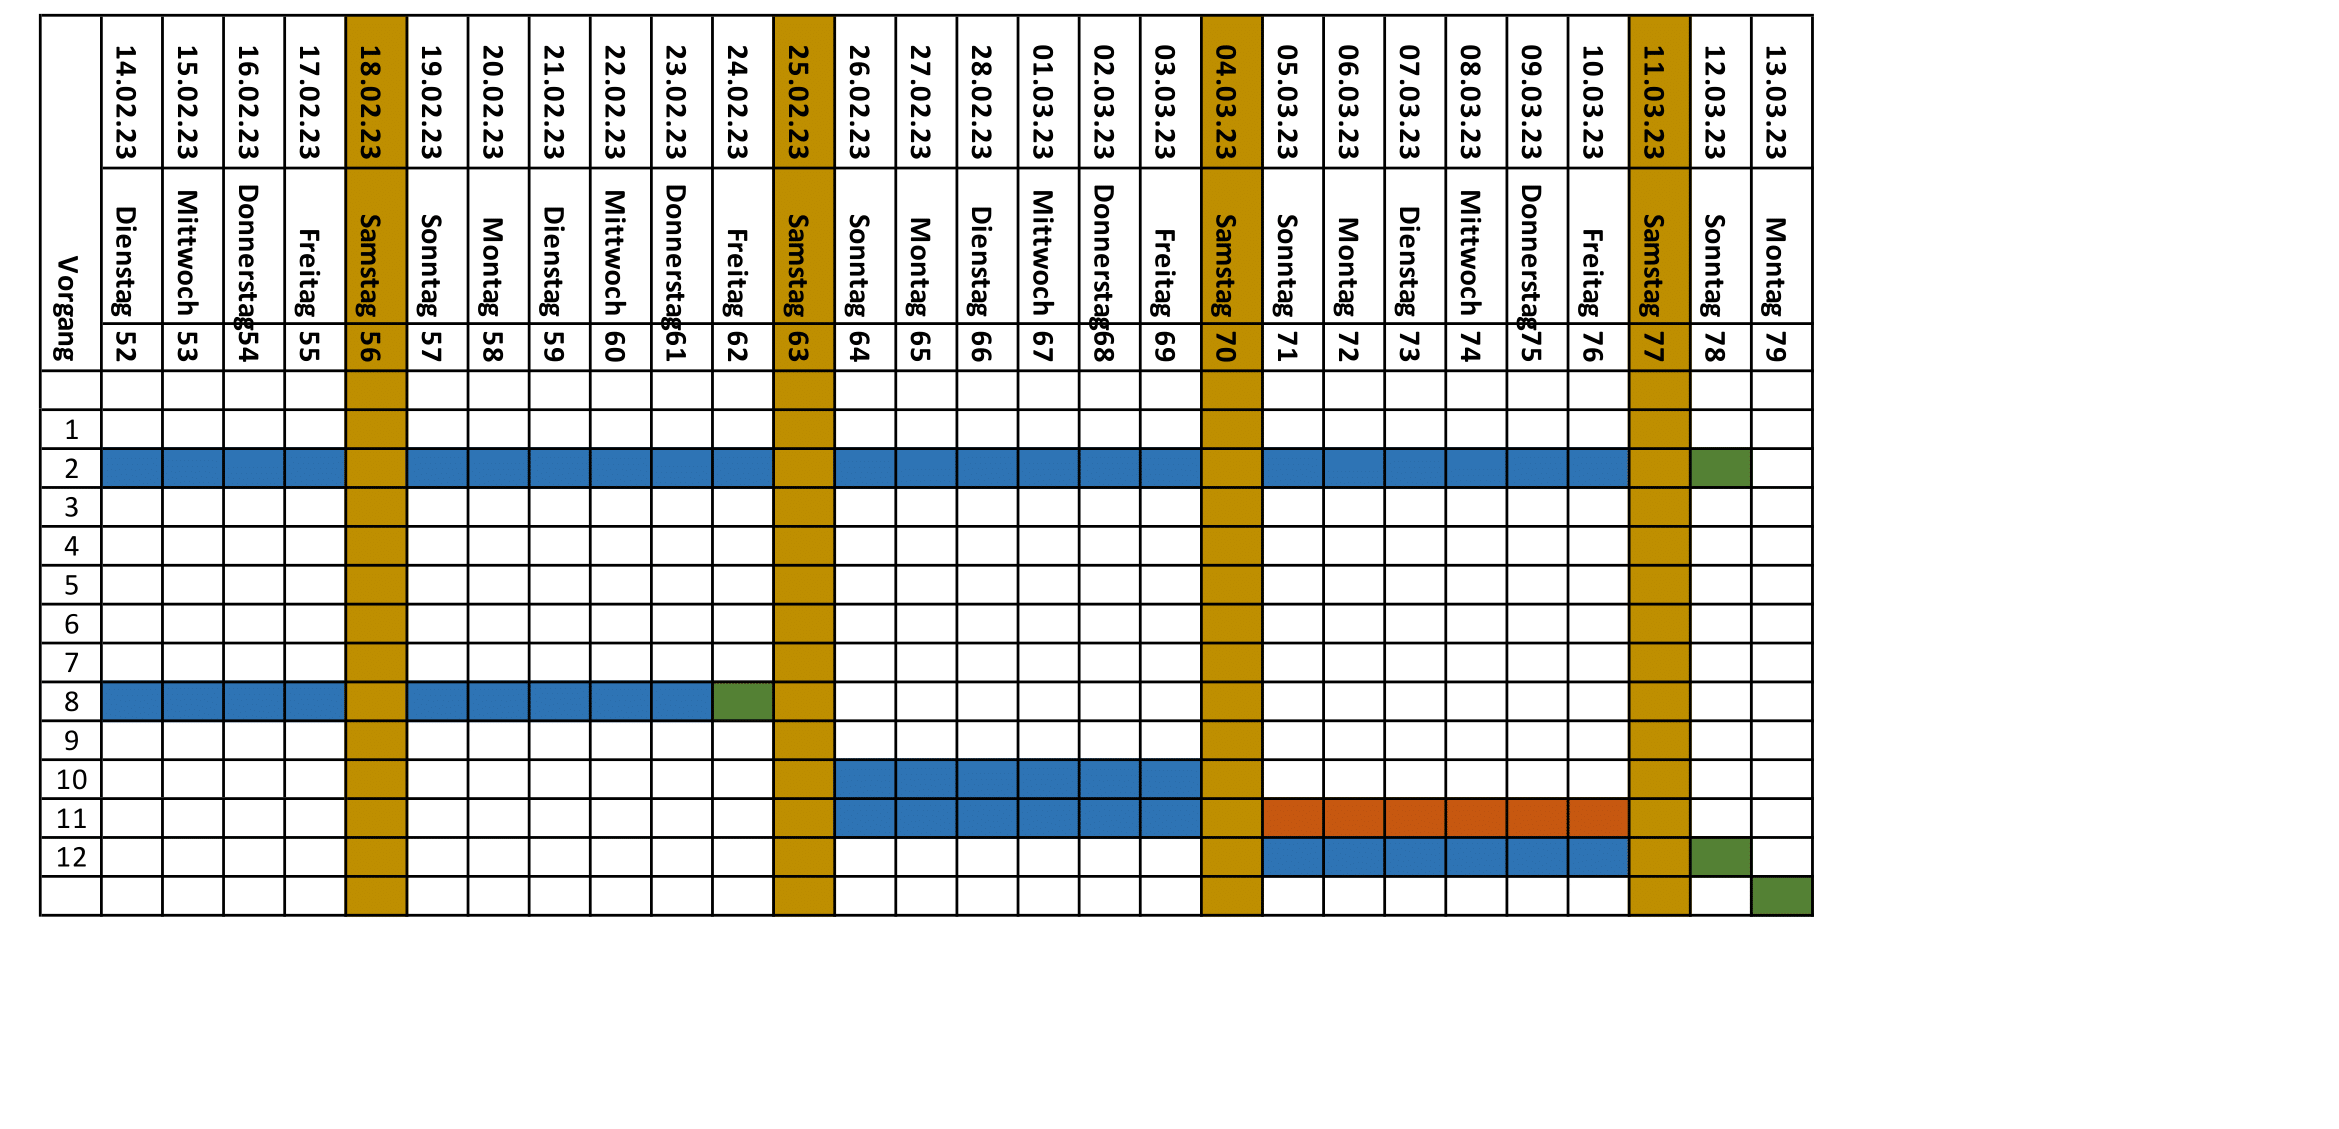
\includegraphics[width=1\linewidth]{Gantt-3.png}
\caption{Zeitliche Planung Teil 3/3}
\label{gantt3}
\end{sidewaysfigure}